\documentclass[conference]{IEEEtran}
\IEEEoverridecommandlockouts
% The preceding line is only needed to identify funding in the first footnote. If that is unneeded, please comment it out.
\usepackage{cite}
\usepackage{amsmath,amssymb,amsfonts}
\usepackage{algorithmic}
\usepackage{graphicx}
\graphicspath{{images/}}
\usepackage{textcomp}
\usepackage{xcolor}
\usepackage{float}
\usepackage{hyperref}
\def\BibTeX{{\rm B\kern-.05em{\sc i\kern-.025em b}\kern-.08em
    T\kern-.1667em\lower.7ex\hbox{E}\kern-.125emX}}
    
\begin{document}

\title{HyGen: Generative Map Creation for Hytale\\
}

\author{\IEEEauthorblockN{Brian Bowers}
\IEEEauthorblockA{\textit{Department of Computer Science} \\
\textit{Loyola Marymount University}\\
Los Angeles, USA \\
bbowers3@lion.lmu.edu}
\and
\IEEEauthorblockN{August Wetterau}
\IEEEauthorblockA{\textit{Department of Computer Science} \\
\textit{Loyola Marymount University}\\
Los Angeles, USA \\
awettera@lion.lmu.edu}
\and
\IEEEauthorblockN{Thomas Rife}
\IEEEauthorblockA{\textit{Department of Computer Science} \\
\textit{Loyola Marymount University}\\
Los Angeles, USA\\
trife@lion.lmu.edu}
}

\maketitle

\begin{abstract}
Map generation, often referred to as procedural generation, is crucial for modern game development. While some maps are fixed, others are uniquely generated on the fly, typically used in open-world games that have a large explorable area. \textit{Hytale} is a fantasy sandbox role-playing game (RPG) that has gained popularity recently, in part due to its built-in tools for animation, modeling, and scripting that allow for accessible modding. Following the application track, we developed a learned generative model that generates map layouts for the game \textit{Hytale}.
\end{abstract}

% \begin{IEEEkeywords}
% component, formatting, style, styling, insert
% \end{IEEEkeywords}


% --------------------- Problem statement and Motivation ----------------------
\section{Problem Statement and Motivation}

Video games with large, explorable maps typically utilize procedural generation. Instead of having each map hand-designed by humans, an algorithm is used. These algorithms use noise functions to generate unique terrain composed of similar features. Procedural generation is used in the game \textit{No Man's Sky} to generate 18 quintillion planets, ensuring players never need to stop exploring. \textit{Minecraft} uses procedural generation combined with a random seed number to generate virtually endless worlds, which can be recreated by any player with the seed. However, the limitation with traditional procedural generation approaches is that often players have no input on what terrain is created. 

\textit{Hytale}, a block-based game similar to \textit{Minecraft}, attempts to let designers have more control over the procedural generation process. Their \textit{World Gen V2} system allows specific patterns to be implemented by players and designers, which can be used to ensure, for example, that glowing mushrooms only appear in sheltered areas \cite{hytale_world_generation_2026}. While these rules can be an effective way to allow players to create custom mods and maps, it still requires users to handcraft these patterns. This is not only time-consuming, but also knowledge-intensive.

A popular feature of \textit{Hytale}, and other similar games, is to allow players to make modifications to the basic game, called ``mods". A few popular \textit{Hytale} mods include boss fights, player-vs-player (PvP) arenas, and dungeon escape quests \cite{curseforge_hytale_2026}. Designing unique and tailored maps for each of these mods is the main limiting factor preventing players from contributing to the game. We decided to address this problem by creating a learned generative model that can generate maps following users' natural language instructions. With our project, users can describe any map they can imagine, and it will be automatically generated for them. 

% --------------------- System Design and Architecture ----------------------
\section{System Design and Architecture}

\subsection{Project Overview}
Our first approach was based on the intuition that map generation, using height maps, is very similar to image generation. Firstly, we decided to experiment with image generation models, including a variational auto-encoder (VAE) and a diffusion model. We trained these models on a procedurally generated dataset. While this produced decent results, we still wanted to create more playable and cohesive maps. To achieve this, we switched to a dataset of scraped maps, which contained more realistic terrain. Finally, we created a hybrid model that outperformed the traditional models. Finally, we implemented our model as a mod in \textit{Hytale}, allowing users to create their own maps.

\subsection{First Approach}
We were unable to find any available datasets containing the data from \textit{Hytale} that we needed. Therefore, we had to create our own dataset. To do this, we used rule-based generation to create maps from seven different archetypes. Each of these archetypes used handcrafted rules designed by us, which led to them being composed of simple designs. Each map involved some random variation, but maps within the same archetype were quite similar. Specifically, the dataset was composed of heightmaps, meaning that they were 2-dimensional arrays where each value represents the height of the topmost block.

Using this dataset, we were able to train a VAE and generate new heightmaps by sampling from the latent space. The results from the VAE were quite blurry, as most of the sharp lines and defining features had been smoothed out. In addition, almost all the maps featured a circular pattern in the middle. This is likely due to the fact that we may have introduced an unintended bias into the dataset, as five of the seven archetypes featured circular shapes in the middle.

We then built a diffusion model, hoping it could address some of the limitations of the VAE. We found that the diffusion model generated much sharper images. In addition, it was able to faithfully capture the less represented archetypes present in our dataset. More importantly, diffusion models can be conditioned on text embeddings through cross-attention mechanisms, which was crucial for allowing players to control the terrain generation.

Additional details of our first approach can be found in our \href{https://github.com/cmsi5998-spring2026/project-final_project_thomas_august_brian/blob/main/progress/5998_GenAI_Final_Project_Progress.pdf}{progress report}.

\begin{figure*}
    \centering
    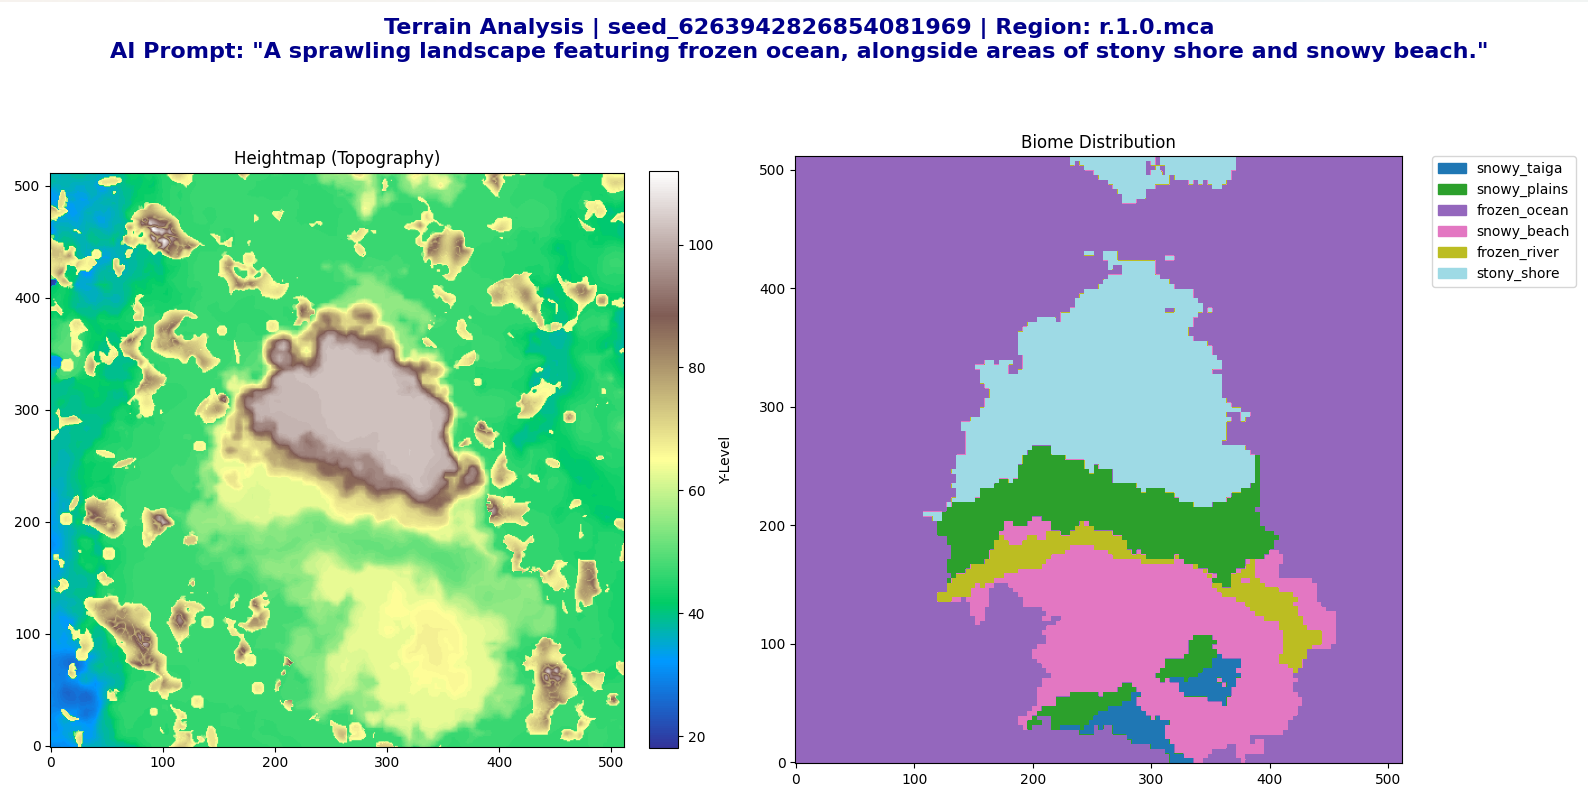
\includegraphics[width=0.9\linewidth]{dataset.png}
    \caption{Example from our final dataset.}
    \label{fig:dataset}
\end{figure*}

\subsection{Second Approach}
When we implemented some of the generated maps from the first approach in game, we saw that they contained unrealistic features that would lead to the game being unplayable. These included noise in places that should be flat, terrain that was incredibly steep, and cut-off features. We hypothesized that part of the problem was due to our procedurally generated dataset. We implemented samples from our dataset in game, and found that while the heightmaps looked good, the actual in game maps were quite poor.

To address this, we decided to build a new dataset, one that was actually based on real terrain in game. Essentially, games such as \textit{Minecraft} and \textit{Hytale}, have much more advanced procedural generation techniques, which we could not compete with. Therefore, it made sense to use their much better procedures to create a dataset. We decided to scrape maps from \textit{Minecraft} because it contains a player-built mod called \textit{Tectonic} \cite{tectonic_curseforge_2026}. This mod recreates terrain-shaping in Minecraft, using more advanced functional noise programming and hardcoded rules. We chose this mod because it has land consolidation (land is grouped together in similar biomes), elevation blending (reduces sharp edges and gains in elevation), and biome smoothing (biomes switch gradually from one another). In addition, it contains aesthetic updates such as coastal cliffs, rolling dunes, and mountain belts. 

We then implemented a script to build a dataset containing scraped map features. Firstly, it generated a random seed, which let us load a new map in the \textit{Tectonic} mod. Then we extracted all blocks within a 100 chunk radius (in \textit{Minecraft} one chunk is 16 blocks). From those blocks, we removed artifacts such as trees, grass, and structures. This left us with a bare terrain that we then chunked up into several 256 by 256 blocks. These patches were then converted into a heightmap. In addition, we also extracted the biome type and created a matching biome distribution map. Then, we used the map metadata to create a text label, representing the natural language input users would give to generate that terrain. An example from our dataset is shown in Figure~\ref{fig:dataset}.

\subsection{Hybrid Approach}
While our automated data pipeline provided an unlimited amount of training data, our main design constraint was the training time. Additionally, diffusion models are very slow due to the gradual denoising process, which we experienced firsthand with our diffusion model from our first approach.

Our main design choice was to use a "warm start", meaning that instead of the diffusion model having to generate images from completely random noise, it would be given a starting point. To accomplish this, we procedurally generated a macro world map, derived from the user prompt. By giving a global representation, the model learns to tune the more fine-grained details, instead of having to learn to generate from scratch.

Furthermore, we used a VAE to compress the map before it is passed into the main diffusion model. This reduced the training time of the diffusion model significantly, in part because it reduces the dimensionality of the diffusion model. In addition, creating a latent representation can help the model by eliminating information that is not useful or redundant. This can help the model learn semantic features better.

We decided to use a Conditional Diffusion U-Net \cite{ronneberger2015u} as our main diffusion model, because for terrain generation, large-scale structure and fine-grained details must both be maintained. U-Nets excel at this, due to their encoder-decoder structure and skip connections. Furthermore, the U-Net can be conditioned on the text-embeddings and biome information to generate terrain that aligns with user input.

Finally, we realized that the U-Net was outputting terrain chunks whose borders did not match, which led to visible seams between neighboring chunks. To address this issue, we added a ControlNet \cite{zhang2023adding}, which provides spatial conditioning based on the borders of the macro world map. This helps the model to generate terrain that complements its surroundings.

The architecture for the first part of our model, the Macro Terrain Generator, is shown in Figure~\ref{fig:arch}.

\begin{figure}[ht]
    \centering
    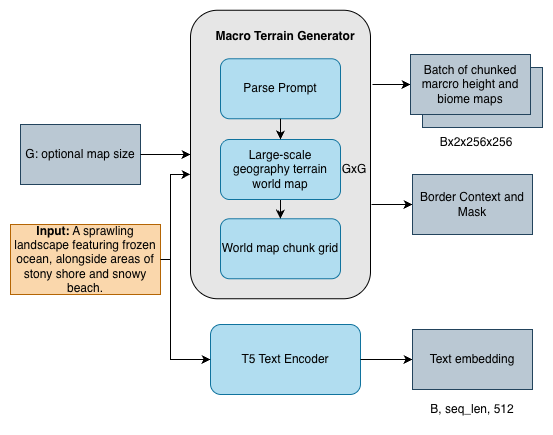
\includegraphics[width=0.85\linewidth]{HyGen.png}
    \caption{Macro Terrain Generator.}
    \label{fig:arch}
\end{figure}

The input into our system is a natural language prompt provided by the user. The prompt is fed to our Macro Terrain Generator, which uses a semantic parser to identify the global terrain archetype. From this classification, a macro low-resolution world map is created. This map contains global features such as mountain belts and canyons, and is used as the starting point for our diffusion process. Additionally, the user can specify the size of the final output map. This means that the generated Macro Terrain world map size is variable. To address this, we chunk up the world map, resulting in a batch of 256 by 256 patches. When chunking up the world map, we use a sliding window, since it preserves contextual information between neighboring chunks. From each, we generate a heightmap and a matching biome map. We also extract border context and a border mask, containing additional information about the terrain features of adjacent chunks. Additionally, the user prompt is passed to a T5 Text Encoder, which generates a text embedding.

The batched 256 by 256 height and biome maps, the border context, and text embedding are directly used in the next steps of the model, shown in Figure~\ref{fig:arch2}.

\begin{figure}[ht]
    \centering
    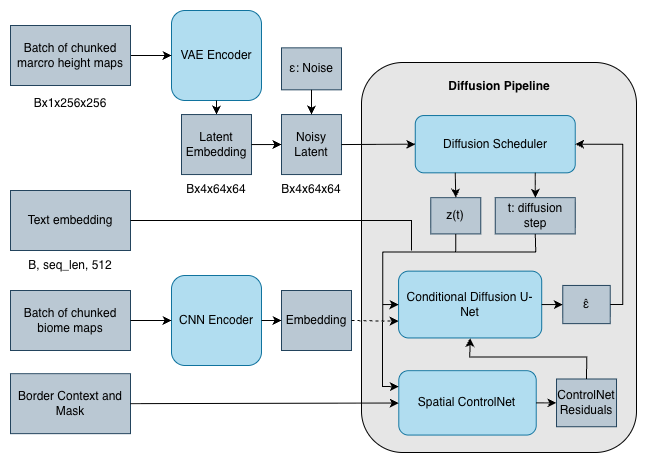
\includegraphics[width=0.85\linewidth]{HyGen2.1.png}
    \caption{Diffusion Pipeline.}
    \label{fig:arch2}
\end{figure}

Firstly, we pass the batched height maps to a VAE, which compresses the 256 by 256 patches into a smaller 64 by 64 latent dimension. Then, random noise (\(\epsilon\)) is added to the latent embedding, resulting in the noisy latent. This is the direct input into our diffusion process, where the added noise will gradually be refined. Similarly, the biome maps are passed to a CNN encoder, which results in an embedding that is also used in the diffusion pipeline. However, we do not add any noise to the biome embedding, as this is used as conditioning in our diffusion model. In addition, the border context and the user prompt embedding are passed into the diffusion pipeline.

The diffusion pipeline is composed of three systems.

\subsubsection{Diffusion Scheduler}
This part is responsible for controlling the diffusion timestep, \(t\), and handling the latent state. At each \(t\), the diffusion scheduler passes the latent state and the timestep to both the U-Net and the ControlNet. Having a shared timestep is crucial for the synchronization of the two diffusion models. The scheduler then takes the output of the U-Net, which is predicted noise (\(\hat{\epsilon}\)), and subtracts the noise from the previous latent state. This process is continued until the maximum number of steps is reached, and the final latent state is output from the diffusion pipeline.

\subsubsection{Conditional Diffusion U-Net}
The input to the U-Net is the latent state from the scheduler, the diffusion step \(t\), the text embedding from the user prompt, the biome embedding, and the residuals from the ControlNet. A U-Net is ideal because it is a specialized convolutional neural network, and our terrain heightmaps can be thought of as patches of single-channel (black and white) images. The encoder in the U-Net downsamples each noisy patch using convolutional layers, which enables the model to learn large-scale features. The decoder in the U-Net then does up-sampling, reconstructing spatial details. In addition, skip connections help to ensure that the model does not forget details from the start of the process. Conditioning on the text embedding ensures that, over time, the noise is shaped to align with the user prompt. In addition, the U-Net can optionally receive a biome embedding, which is created by using a CNN encoder on the biome map. This biome embedding helps the model by guiding the terrain generation, as it provides clear separation between mountains, rivers, etc.

\subsubsection{Spatial ControlNet}
The input to the ControlNet is the shared diffusion timestep and latent state. The main job of the ControlNet is to output residuals, which tell the U-Net information about what features to add so that the chunks match their neighbors. To do this, it must be at the same time step as the U-Net, as otherwise it would be providing information about past states that may not be applicable to the current state. To help the ControlNet output useful residuals, it is conditioned on the user prompt text embedding, the border context, and the border mask. The border context and mask provide terrain boundaries of the surrounding regions. This helps the U-Net to ensure that the generated chunks match and there are no visible seams between bordering chunks, allowing the map to be more geographically consistent and playable. 

To enhance the diffusion models' adherence to the user prompt, we use Classifier-Free Guidance (CFG). This means that during training, we would occasionally remove the T5 prompt. This forces the diffusion model to learn two noise predictions, which amplifies the user prompt. In addition, we used Exponential Moving Average (EMA) when updating the model weights. This helped to stabilize the training process and helps to ensure the generated terrain is realistic.

\begin{figure}[ht]
    \centering
    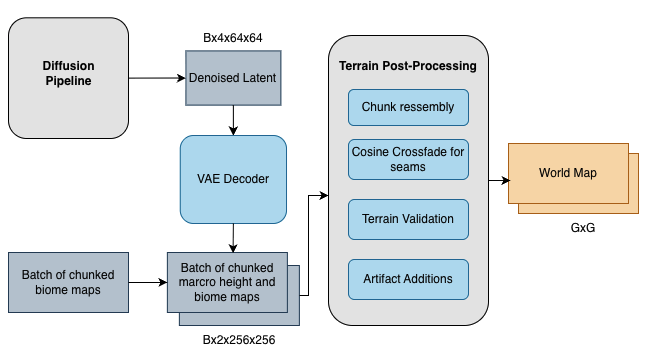
\includegraphics[width=0.85\linewidth]{HyGen3.png}
    \caption{Terrain Post-Processing.}
    \label{fig:arch3}
\end{figure}

The denoised latent is the final output of the diffusion pipeline. This is passed through the VAE decoder, which results in the final heightmap chunks of 256 by 256. We then add back in the biome chunks to the heightmaps, which becomes the input to our Terrain Post-Processing module, shown in Figure~\ref{fig:arch3}. The main goal of this module is to reassemble the chunks to recreate the world map. Each chunk has an overlapping window, which, due to the Control-Net, should have matching terrain. However, since there are two different generated terrain values for the borders, we need to decide which ones to use. To do this, we apply a cosine crossfade to ensure we are using parts from both boarding chunks. Doing this helps to ensure that the chunks look natural and that there are no visible grid patterns in the world map from where the chunks were separated. Furthermore, we use a validation step to ensure that there are no issues in the final world map, such as floating terrain, impossible cliffs, and biome inconsistencies. This is the final terrain map that is output from the world map. Optionally, we also add in some artifacts, or terrain decorations, such as trees, plants, cacti, flowers, snow, etc. We allowed users to choose whether they wanted these artifacts, as often users will want to implement these themselves, and our focus is just on generating the actual terrain.

% --------------------- Generative AI Integration Details ----------------------
\section{Generative AI Integration Details}
Our project focuses on solving an inherently generative process, creating terrain maps. While traditional procedural generation methods are deterministic and hand-crafted, we applied more advanced generative models to the problem. After exploring several different approaches, we settled on a hybrid method that procedurally generates a starting point, which is then compressed by a VAE and input into our diffusion model. We used a diffusion model as our main source for creating maps, since it allowed us to condition the outputs on the user input. This allows users to have more control over the generated terrain than traditional procedural generative approaches.

% --------------------- Evaluation and User Feedback ----------------------
\section{Evaluation and User Feedback}

To evaluate our system, we compared the outputs from each stage of development, including the rule-based procedural generator, the VAE, the standalone diffusion model, and the final hybrid architecture. Our evaluation focused primarily on terrain realism, biome coherence, prompt adherence, and overall playability when implemented in game environments.

The rule-based procedural generator was effective for rapidly producing large quantities of training data, but the generated terrain often appeared repetitive and unrealistic when imported into game environments. Because the terrain archetypes relied on hand-crafted rules, many maps shared similar structures and lacked the natural variation typically found in open-world games. While these maps were useful for early experimentation, they did not provide sufficient realism for playable environments.

The VAE improved terrain diversity by learning latent representations of the training maps and generating entirely new terrain samples. However, the generated outputs were frequently blurry and lacked sharp terrain transitions. We also observed a recurring circular structure near the center of many generated maps, likely caused by unintended bias in the procedurally generated dataset. Although the VAE was computationally efficient, the resulting terrain often contained unrealistic smoothing and lacked the detailed structure necessary for immersive gameplay.

The standalone diffusion model produced significantly sharper terrain and better preserved local terrain features. In addition, conditioning the diffusion process on text embeddings allowed users to influence terrain generation through natural language prompts. Prompts such as ``mountain canyon biome" and ``snowy valley with rivers" produced outputs that generally aligned with the requested terrain structure. Despite these improvements, the diffusion model introduced several practical issues when maps were implemented in game. Generated chunks frequently contained visible seams at chunk boundaries, abrupt elevation changes, and noisy terrain artifacts that negatively affected gameplay and navigation.

The final hybrid architecture produced the strongest overall results. By combining a procedurally generated macro terrain map with latent diffusion refinement, the system generated terrain that was both more globally coherent and more geographically realistic. The addition of the ControlNet and border conditioning significantly reduced visible seams between neighboring terrain chunks, while the cosine crossfade post-processing further improved terrain continuity. Generated maps contained smoother biome transitions, more natural elevation blending, and fewer terrain discontinuities than previous approaches.

We additionally evaluated the system through in-game testing by importing generated terrain into sandbox environments and manually exploring the resulting worlds. Compared to earlier models, the final hybrid system produced terrain that was substantially easier to navigate and visually consistent. Features such as mountain ranges, coastlines, rivers, and valleys appeared more naturally connected, and the generated terrain was generally more playable without requiring extensive manual correction.

We also collected informal feedback from other players. Users responded positively to the ability to generate terrain using natural language prompts and appreciated the speed at which large maps could be created. Many users viewed the system as a creative assistance tool that could accelerate map prototyping and reduce the amount of repetitive manual terrain work required during mod development. However, users also expressed interest in more fine-grained controls, such as the ability to edit generated terrain interactively or specify the placement of important landmarks and structures. These suggestions motivated several directions for future work.

% --------------------- AI Ethics Reflection ----------------------
\section{AI Ethics Reflection}

The use of generative AI for creative applications raises important ethical considerations about authorship, creativity, and responsible use of resources. Our project focused on generating terrain maps for sandbox-style games, which are traditionally created either manually by designers or procedurally through hand-crafted algorithms. Rather than replacing human creativity, our goal was to create a tool that assists players and mod developers by accelerating the terrain creation process and allowing users to express ideas through natural language prompts.

One important ethical consideration is the relationship between generated outputs and the training data. Because \textit{Hytale} is not yet publicly available, we created our dataset using terrain generated from the \textit{Minecraft} \textit{Tectonic} mod. Importantly, these maps were procedurally generated worlds rather than hand-crafted player creations. This reduces concerns surrounding similar maps to individual artistic works, though that issue could still be present. Our intention was not to reproduce existing worlds, but instead to learn general terrain formation patterns that could be applied to generate entirely new environments.

Another ethical concern involves the role of AI in creative communities. Generative systems can significantly reduce the time required to build large game environments, which may benefit independent developers and players with limited technical experience. However, excessive reliance on automated systems could potentially reduce intentional design choices and homogenize creative content. To address this concern, our system was designed as an assistive tool rather than a fully autonomous replacement for human designers. Users still control the generation process through prompts, biome selection, and optional post-processing decisions, allowing human creativity to remain central to the final result.

Finally, we considered the computational cost associated with modern generative AI systems. Diffusion models are computationally expensive and often require significant training time and hardware resources. Because of these constraints, we intentionally designed a hybrid architecture that combined procedural generation, latent compression through a VAE, and conditional diffusion refinement. This reduced the dimensionality of the generation process and improved training efficiency while still producing realistic terrain outputs. By prioritizing efficiency in the system design, we aimed to reduce unnecessary computational overhead and make the model more accessible for practical use by smaller development teams and modding communities.

% --------------------- Conclusion and Future Work ----------------------
\section{Conclusion}

In this project, we developed \textit{HyGen}, a learned generative AI system for creating terrain maps for the sandbox RPG game \textit{Hytale}. Traditional procedural generation methods are effective for producing large worlds, but they often provide limited control to players and require extensive hand-crafted rules to create specific terrain features. Our goal was to combine the scalability of procedural generation with the flexibility and controllability of modern generative AI models.

Throughout development, we explored several different approaches, including a VAE, a standalone diffusion model, and a final hybrid architecture. While the VAE provided efficient latent representations, it struggled to preserve sharp terrain structure and generated overly smooth outputs. The diffusion model improved realism and prompt adherence, but introduced issues such as terrain seams and inconsistent chunk boundaries. These limitations motivated the development of our hybrid approach, which combined procedural macro terrain generation, latent diffusion refinement, biome conditioning, and ControlNet-based spatial conditioning.

The final system generated terrain that was more coherent, realistic, and playable than earlier approaches. By conditioning generation on natural language prompts, users were able to influence terrain style and biome structure without manually designing maps or writing procedural generation rules. In addition, our chunk blending and border conditioning pipeline significantly reduced visible seams and improved terrain continuity across large generated worlds.

Overall, this project demonstrates how generative AI can be integrated into creative game development workflows to assist players and mod developers in rapidly prototyping large-scale environments. Rather than replacing human creativity, our system acts as a collaborative design tool that helps users transform high-level ideas into explorable game worlds.

\section{Future Work}

While our system was capable of generating coherent and playable terrain maps, there are several areas where the project could be expanded in future work. One major limitation of the current system is that generation occurs primarily at the terrain level using 256 by 256 heightmap chunks. Future versions of the project could focus on generating significantly larger worlds with more detailed global structure, allowing for continent-scale terrain generation with long-distance geographic consistency between regions.

Another important direction would be improving the expressiveness of the natural language interface. Currently, the Macro Terrain Generator relies largely on keyword parsing and predefined terrain archetypes to guide generation. Future systems could instead use a learned semantic classifier or a large language model to better understand more complex prompts and nuanced user intent. This would allow users to specify detailed world characteristics, environmental storytelling elements, or combinations of terrain styles that are difficult to represent using simple keyword-based parsing.

Additionally, our current system focuses primarily on terrain elevation and biome generation. Future work could extend the model to generate environmental details such as trees, vegetation, rivers, caves, structures, villages, dungeons, and other gameplay-relevant landmarks. Incorporating these features would allow the generated worlds to feel more complete and immersive while reducing the amount of manual post-processing required by players and mod developers.

Finally, future iterations of the system could support interactive editing and real-time terrain refinement. Rather than generating an entire world in a single step, users could iteratively modify terrain regions, regenerate specific areas, or provide feedback during generation. This would further position the system as a collaborative creative tool that works alongside players and designers during the world-building process.

\section{Bonus Multi-Modal Integration}

Our project integrates text input into the map generation process. Specifically, our users input a natural language description of the map they want generated, which is then used to guide the map generation. Specifically, user prompts are embedded using T5 and then passed to our U-Net diffusion model to be conditioned on. We faced several technical challenges when implementing this multimodal integration, with most of them focused on having the U-Net generation aligned with the user prompt. One approach that helped was using Classifier Free Guidance (CFG). Additional information about the model and training has also been discussed in greater detail in previous sections.

% \begin{figure}
%     \centering
%     \includegraphics[width=0.85\linewidth]{epoch_20_samples (6).png}
%     \caption{Enter Caption}
%     \label{fig:dif}
% \end{figure}


\bibliographystyle{IEEEtran}
\bibliography{ref}

\end{document}
